\chapter{روش‌شناسی}

\section{انتخاب مدل زبان}

در این بخش، مدل زبانی مناسب برای توسعه چت‌بات آموزشی مورد بررسی قرار گرفت. مدل‌های زبانی مختلفی برای چت‌بات‌ها وجود دارند که هر یک دارای مزایا و معایب خاص خود هستند. برخی از عوامل مهم در انتخاب مدل زبان عبارتند از:

\begin{itemize}
    \item حجم داده‌های آموزشی: مدل‌های زبانی بزرگ‌تر، به داده‌های آموزشی بیشتری نیاز دارند.
    \item سرعت پردازش: مدل‌های زبانی کوچک‌تر، سریع‌تر پردازش می‌شوند.
    \item دقت پاسخ‌دهی: مدل‌های زبانی دقیق‌تر، پاسخ‌های دقیق‌تری ارائه می‌دهند.
\end{itemize}

در این پروژه، از مدل زبان \lr{SpacyNLP xx\_sent\_ud\_sm} استفاده شد. این مدل زبان، یک مدل زبانی کوچک و سریع است که بر روی مجموعه داده‌های بزرگی از متن و کد آموزش دیده است. این مدل زبان، دقت پاسخ‌دهی مناسبی نیز دارد.

\subsection{دلایل انتخاب مدل \lr{SpacyNLP xx\_sent\_ud\_sm}}

دلایل انتخاب مدل \lr{SpacyNLP xx\_sent\_ud\_sm} عبارتند از:

\begin{itemize}
    \item حجم داده‌های آموزشی: این مدل زبان، بر روی مجموعه داده‌های بزرگی از متن و کد آموزش دیده است که این امر، دقت پاسخ‌دهی آن را افزایش می‌دهد.
    \item سرعت پردازش: این مدل زبان، یک مدل زبانی کوچک و سریع است که این امر، آن را برای توسعه چت‌بات‌های آموزشی مناسب می‌سازد.
    \item چند زبانه بودن: این مدل زبان، بر روی مجموعه داده‌هایی از زبان‌های مختلف آموزش دیده است که این امر، آن را برای توسعه چت‌بات‌های آموزشی چند زبانه مناسب می‌سازد.
    \item آموزش بر روی جملات: این مدل زبان، بر روی مجموعه داده‌هایی از جملات آموزش دیده است که این امر، آن را برای توسعه چت‌بات‌های آموزشی که باید به سوالات و درخواست‌های کاربران پاسخ دهند، مناسب می‌سازد.
\end{itemize}

\subsection{نتیجه‌گیری}

مدل \lr{SpacyNLP xx\_sent\_ud\_sm}،  یک مدل زبانی کوچک، سریع، دقیق و چند زبانه است که برای توسعه چت‌بات‌های آموزشی مناسب می‌باشد. این مدل زبان، بر روی مجموعه داده‌های بزرگی از متن و کد آموزش دیده است که این امر، دقت پاسخ‌دهی آن را افزایش می‌دهد. همچنین، این مدل زبان، سریع است که این امر، آن را برای توسعه چت‌بات‌های آموزشی که باید به سرعت پاسخ‌های کاربران را ارائه دهند، مناسب می‌سازد. علاوه بر این، این مدل زبان، بر روی مجموعه داده‌هایی از زبان‌های مختلف آموزش دیده است که این امر، آن را برای توسعه چت‌بات‌های آموزشی چند زبانه مناسب می‌سازد. همچنین، این مدل زبان، بر روی مجموعه داده‌هایی از جملات آموزش دیده است که این امر، آن را برای توسعه چت‌بات‌های آموزشی که باید به سوالات و درخواست‌های کاربران پاسخ دهند، مناسب می‌سازد.

در این بخش، توضیحاتی در مورد معنای حروف و کلمات استفاده شده در نام مدل زبان \lr{SpacyNLP xx\_sent\_ud\_sm} ارائه شده است.

xx : مخفف چند زبانه بودن (multilingual)

sent : مخفف روی جملات آموزش دیدن (sentences)

ud : مخفف \lr{Universal Dependencies}

sm : مخفف کوچک (small)

بنابراین، نام مدل زبان \lr{SpacyNLP xx\_sent\_ud\_sm}، به معنای مدل زبانی کوچک و سریع چند زبانه است که بر روی مجموعه داده‌هایی از جملات با ساختارهای دستوری جهانی آموزش دیده است.

\subsection{\lr{Universal Dependencies (UD)} چیست؟}
یک چارچوب\footnote{Structure} برای نشان دادن دستور زبان (اجزای گفتار، ویژگی‌های صرفی و روابط دستوری) در زبان‌های مختلف است. این چارچوب بر اساس یک مجموعه از روابط دستوری جهانی است که برای توصیف روابط بین کلمات در هر زبانی استفاده می‌شود.

\lr{Universal Dependencies} \cite{2} در سال 2013 توسط یک گروه از محققان از دانشگاه استنفورد، دانشگاه آکسفورد و دانشگاه کمبریج ایجاد شد. این چارچوب به سرعت مورد پذیرش قرار گرفت و اکنون برای ایجاد بانک‌های درختی برای بیش از 100 زبان استفاده می‌شود.

UD مزایای متعددی دارد. این یک چارچوب انعطاف‌پذیر است که می‌تواند برای توصیف ساختارهای دستوری پیچیده در زبان‌های مختلف استفاده شود. این یک چارچوب باز است که به محققان اجازه می‌دهد روابط دستوری جدیدی را اضافه کنند. و این یک چارچوب رایگان است که برای همه در دسترس است.

UD در طیف گسترده‌ای از برنامه‌های کاربردی استفاده می‌شود. از جمله:

\begin{itemize}
\item پردازش زبان طبیعی (NLP): UD برای توسعه ابزارهای NLP مانند چت‌بات‌ها، ترجمه ماشینی و تشخیص گفتار استفاده می‌شود.
\item آموزش زبان: UD برای توسعه منابع آموزشی مانند فرهنگ لغات و دستور زبان استفاده می‌شود.
\item تحقیقات زبانشناسی: UD برای مطالعه ساختار دستوری زبان‌های مختلف استفاده می‌شود.
\end{itemize}

UD یک چارچوب مهم برای پردازش زبان طبیعی و تحقیقات زبانشناسی است. این چارچوب به محققان این امکان را می‌دهد تا ساختار دستوری زبان‌های مختلف را به روشی استاندارد و سازگار توصیف کنند.


\section{آماده‌سازی داده‌ها و ایجاد مجموعه داده‌های آموزشی}


در این بخش، داده‌های مورد نیاز برای آموزش چت‌بات Rasa از طریق شیوه نامه آموزشی ۱۴۰۰ دانشگاه فردوسی مشهد تهیه شد. این شیوه نامه شامل تعاریف، ماده ها و تبصره های مختلف مربوط به امور آموزشی دانشگاه است. داده‌ها به صورت پرسش و پاسخ تهیه شدند و به صورت زیر دسته‌بندی شدند:

\begin{itemize}
    \item تعاریف: تعاریف مختلف مربوط به امور آموزشی دانشگاه در قالب پرسش و پاسخ تهیه شدند. به عنوان مثال، پرسش "دانشجو چیست؟" با پاسخ "شخصی که در یکی از دانشگاه‌های ایران در حال تحصیل است" همراه شد.
    \item ماده ها: ماده های مختلف شیوه نامه آموزشی به صورت پرسش و پاسخ تهیه شدند. به عنوان مثال، پرسش "ماده 1 شیوه نامه آموزشی چیست؟" با پاسخ "تعریف دانشجو" همراه شد.
    \item تبصره ها: تبصره های مختلف شیوه نامه آموزشی به صورت پرسش و پاسخ تهیه شدند. به عنوان مثال، پرسش "تبصره 1 ماده 1 شیوه نامه آموزشی چیست؟" با پاسخ "شرایط پذیرش دانشجو در دانشگاه" همراه شد.
\end{itemize}

در مجموع، پرسش و پاسخ های زیادی برای آموزش چت‌بات تهیه شد. این پرسش و پاسخ ها به صورت دستی تهیه شدند و سپس با استفاده از Rasa به صورت مجموعه داده‌های آموزشی تبدیل شدند.

\subsection{محدودیت‌های مجموعه داده‌های آموزشی}


مجموعه داده‌های آموزشی تهیه شده دارای برخی محدودیت‌ها است. یکی از محدودیت‌ها این است که این مجموعه داده‌ها فقط شامل تعاریف، ماده ها و تبصره های شیوه نامه آموزشی است. بنابراین، ممکن است پاسخ‌های چت‌بات برای برخی پرسش‌های خارج از این محدوده، دقیق نباشد.

محدودیت دیگر این است که مجموعه داده‌های آموزشی به صورت دستی تهیه شده است. این امر ممکن است باعث شود که برخی پرسش و پاسخ ها ناقص یا دارای اشکال باشند.

\subsection{راهکارهای بهبود مجموعه داده‌های آموزشی}

برای بهبود مجموعه داده‌های آموزشی، می‌توان اقدامات زیر را انجام داد:

مجموعه داده‌ها را با پرسش و پاسخ‌های بیشتری از منابع مختلف، مانند وب سایت‌های دانشگاهی، تکمیل کرد.
از نرم‌افزارهای خودکار برای شناسایی و اصلاح اشکالات موجود در مجموعه داده‌ها استفاده کرد.
با انجام این اقدامات، می‌توان مجموعه داده‌های آموزشی را دقیق‌تر و کامل‌تر کرد و عملکرد چت‌بات را بهبود بخشید.


\section{توسعه چت‌بات Rasa}

پس از آماده‌سازی داده‌های آموزشی، می‌توان چت‌بات را توسعه داد. چت‌بات Rasa از یک چارچوب توسعه چت‌بات متن باز استفاده می‌کند. این چارچوب شامل ابزارها و کتابخانه‌هایی برای توسعه چت‌بات‌های آموزشی است.

در این پروژه، از چارچوب Rasa استفاده شده است. برای توسعه چت‌بات، ابتدا باید یک پروژه Rasa ایجاد شود. سپس، مدل زبان انتخاب‌شده به پروژه اضافه می‌شود. در مرحله بعد، مجموعه داده‌های آموزشی به پروژه اضافه می‌شود.

Rasa از یک فرآیند آموزش خودکار برای آموزش چت‌بات استفاده می‌کند. این فرآیند به چت‌بات اجازه می‌دهد تا از مجموعه داده‌های آموزشی یاد بگیرد و توانایی خود را در پاسخ به سوالات و درخواست‌های کاربران بهبود بخشد.

\section{ادغام Rocket.Chat}

ادغام Rocket.Chat با Rasa یک راه عالی برای افزودن قابلیت‌های چت‌بات AI به پلتفرم چت سازمانی شماست. با این ادغام، می‌توانید از Rasa برای ساخت چت‌بات‌هایی استفاده کنید که می‌توانند به سوالات و درخواست‌های کاربران پاسخ دهند، پشتیبانی مشتری ارائه دهند، یا حتی کارهایی مانند جمع‌آوری داده‌ها یا برنامه‌ریزی کارها را انجام دهند.

\section{راه‌اندازی}

برای راه‌اندازی این پروژه بر روی سیستم خود می‌توانید مراحل این قسمت را دنبال کنید.\footnote{توجه تمامی مراحل نصب با فرض این که شما در یک ترمینال linux-based هستید بیان شده‌اند.}

\subsection{راه‌اندازی Rocket.Chat}

\subsubsection{نصب پیشنیاز‌ها}

در ابتدا شما باید npm را نصب کنید.

\begin{latin}
    \begin{minted}[
    framesep=2mm,
    baselinestretch=1.2,
    bgcolor=LightGray,
    fontsize=\footnotesize,
    linenos
    ]{bash}
    npm install npm@latest -g
    \end{minted}
\end{latin}


توجه داشته باشید که باید Node نسخه ۱۴ را داشته باشید.

برای بررسی نسخه Node خود می‌توانید از دستور ذیل استفاده کنید.

\begin{latin}
    \begin{minted}[
    framesep=2mm,
    baselinestretch=1.2,
    bgcolor=LightGray,
    fontsize=\footnotesize,
    linenos
    ]{bash}
    node -v
    \end{minted}
\end{latin}


اگر نسخه Node شما ۱۴ نبود با دستور زیر آن را به ۱۴ ببرید.

\begin{latin}
    \begin{minted}[
    framesep=2mm,
    baselinestretch=1.2,
    bgcolor=LightGray,
    fontsize=\footnotesize,
    linenos
    ]{bash}
    sudo n 14.21.3
    \end{minted}
\end{latin}


همچنین شما برای استفاده از Rocket.Chat نیاز به نصب meteor دارید.

برای نصب meteor می‌توانید از دستور زیر استفاده کنید.

\begin{latin}
    \begin{minted}[
    framesep=2mm,
    baselinestretch=1.2,
    bgcolor=LightGray,
    fontsize=\footnotesize,
    linenos
    ]{bash}
    npm install -g meteor
    \end{minted}
\end{latin}

اگر برای نصب meteor مشکلی بود می‌توانید از دستورات زیر استفاده کنید.

\begin{latin}
    \begin{minted}[
    framesep=2mm,
    baselinestretch=1.2,
    bgcolor=LightGray,
    fontsize=\footnotesize,
    linenos
    ]{bash}
    curl https://install.meteor.com/\?release\=2.13.3 | sh
    \end{minted}
\end{latin}

\begin{latin}
    \begin{minted}[
    framesep=2mm,
    baselinestretch=1.2,
    bgcolor=LightGray,
    fontsize=\footnotesize,
    linenos
    ]{bash}
    sudo npm install -g meteor --unsafe-perm
    \end{minted}
\end{latin}

در آخر باید yarn را برای استفاده از Rocket.Chat نصب کنید.

برای نصب yarn در \lr{Arch linux} می‌توان از دستورات زیر استفاده کرد.

\begin{latin}
    \begin{minted}[
    framesep=2mm,
    baselinestretch=1.2,
    bgcolor=LightGray,
    fontsize=\footnotesize,
    linenos
    ]{bash}
    sudo npm install --global yarn 
    \end{minted}
\end{latin}

اگر از Arch استفاده نمی‌کنید در دستور زیر به جای \lr{pacman -S} از پکیج منیجر مربوط به توزیع خود استفاده کنید.

\begin{latin}
    \begin{minted}[
    framesep=2mm,
    baselinestretch=1.2,
    bgcolor=LightGray,
    fontsize=\footnotesize,
    linenos
    ]{bash}
    sudo pacman -S yarn 
    \end{minted}
\end{latin}

در این مرحله باید Rocket.Chat را از مخزن رسمی اش دریافت کنید که می‌توانید با استفاده از دستور زیر این کار را انجام دهید.

\begin{latin}
    \begin{minted}[
    framesep=2mm,
    baselinestretch=1.2,
    bgcolor=LightGray,
    fontsize=\footnotesize,
    linenos
    ]{bash}
    git clone https://github.com/RocketChat/Rocket.Chat.git
    \end{minted}
\end{latin}

سپس برای نصب پیشنیاز‌های Rocket.Chat در پوشه ای که Rocket.Chat را Clone کرده اید دستور زیر را وارد کنید.

این پوشه معمولا Rocket.Chat نام دارد.

\begin{latin}
    \begin{minted}[
    framesep=2mm,
    baselinestretch=1.2,
    bgcolor=LightGray,
    fontsize=\footnotesize,
    linenos
    ]{bash}
    yarn
    \end{minted}
\end{latin}

و در نهایت برای شروع استفاده از Rocket.Chat می‌توانید از یکی از دستورات زیر استفاده کنید.

 دستور زیر همه پکیج ها را اجرا می‌کند.
\begin{latin}
    \begin{minted}[
    framesep=2mm,
    baselinestretch=1.2,
    bgcolor=LightGray,
    fontsize=\footnotesize,
    linenos
    ]{bash}
    yarn dev
    \end{minted}
\end{latin}

دستور زیر فقط \lr{meteor (front and back)} به همراه پکیج های از پیش ساخته شده را اجرا می‌کند.

\begin{latin}
    \begin{minted}[
    framesep=2mm,
    baselinestretch=1.2,
    bgcolor=LightGray,
    fontsize=\footnotesize,
    linenos
    ]{bash}
    yarn dsv
    \end{minted}
\end{latin}

\subsection{راه‌اندازی Rasa}

\warning\;هشدار

نسخه های پشتیبانی شده \lr{Python3}

در حال حاضر، Rasa از نسخه های زیر Python پشتیبانی می کند:

\lr{3.7، 3.8، 3.9 و 3.10}. لطفا توجه داشته باشید که \lr{Python 3.10} فقط برای نسخه های \lr{3.4.x} و بالاتر پشتیبانی می شود. علاوه بر این، نصب Rasa روی \lr{Apple Silicon} با \lr{Python 3.10} در نسخه \lr{3.4.x}کار نمی کند اما از \lr{3.5.x} به بعد پشتیبانی خواهد شد.

\subsubsection{نصب پیشنیاز‌ها}

در ابتدا برای استفاده از Rasa باید پایتون نسخه \lr{۳.۱۰} را روی سیستم نصب کنیم.

بعد از نصب پایتون باید \lr{virtual environment} پایتون نصب شود برای نصب این محیط از دستور زیر استفاده می‌کنیم.

\begin{latin}
    \begin{minted}[
    framesep=2mm,
    baselinestretch=1.2,
    bgcolor=LightGray,
    fontsize=\footnotesize,
    linenos
    ]{bash}
    python3.10 -m venv .venv
    \end{minted}
\end{latin}

برای رفتن به \lr{virtual environment} از دستور زیر استفاده می‌کنیم

\begin{latin}
    \begin{minted}[
    framesep=2mm,
    baselinestretch=1.2,
    bgcolor=LightGray,
    fontsize=\footnotesize,
    linenos
    ]{bash}
    source .venv/bin/activate
    \end{minted}
\end{latin}

بعد از رفتن به \lr{virtual environment} با دستور زیر چک می‌کنیم که نسخه پایتون ما درست است یا خیر

\begin{latin}
    \begin{minted}[
    framesep=2mm,
    baselinestretch=1.2,
    bgcolor=LightGray,
    fontsize=\footnotesize,
    linenos
    ]{bash}
    python -V
    \end{minted}
\end{latin}

و همینطور با دستور زیر مطمئن می‌شویم که pip نصب شده است یا خیر

\begin{latin}
    \begin{minted}[
    framesep=2mm,
    baselinestretch=1.2,
    bgcolor=LightGray,
    fontsize=\footnotesize,
    linenos
    ]{bash}
    pip -V
    \end{minted}
\end{latin}

سپس با دستور زیر شروع به نصب Rasa و ارتقای pip می‌کنیم. اجرای این دستور ممکن است کمی زمان‌بر باشد.

\begin{latin}
    \begin{minted}[
    framesep=2mm,
    baselinestretch=1.2,
    bgcolor=LightGray,
    fontsize=\footnotesize,
    linenos
    ]{bash}
    python -m pip install --upgrade pip rasa
    \end{minted}
\end{latin}

برای دیدن سوییچ هایی که Rasa در اختیار شما قرار می‌دهد می‌توانید از دستور زیر استفاده کنید.

\begin{latin}
    \begin{minted}[
    framesep=2mm,
    baselinestretch=1.2,
    bgcolor=LightGray,
    fontsize=\footnotesize,
    linenos
    ]{bash}
    python -m rasa --help
    \end{minted}
\end{latin}

برای ساخت یک پروژه جدید Rasa از دستور زیر استفاده می‌کنیم در حین اجرای این دستور Rasa از شما سوالاتی راجع به پروژه می‌پرسد که پس از پاسخ به آن‌ها پروژه ساخته خواهد شد.

\begin{latin}
    \begin{minted}[
    framesep=2mm,
    baselinestretch=1.2,
    bgcolor=LightGray,
    fontsize=\footnotesize,
    linenos
    ]{bash}
    python -m rasa --init
    \end{minted}
\end{latin}

بعد از وارد شدن به \lr{virtual environment} تمام دستورات تا اینجا در این محیط اجرا می‌شوند.

\subsection{اتصال Rocket.Chat و Rasa}

\subsubsection{تنظیمات کاربر ربات در Rocket.Chat}

در Rocket.Chat یک کاربر ربات Rasa ایجاد کنید. می توانید به صورت دستی به Rocket.Chat وارد شوید و یک کاربر ربات را از طریق صفحه مدیریت کاربر ایجاد کنید یا می توانید از اسکریپت زیر برای ایجاد کاربر ربات استفاده کنید.
برای ایجاد ربات Rasa دستور زیر را اجرا کنید.

توجه: لطفا نام کاربری و رمزعبور مدیر Rocket.Chat و کاربر ربات را به ترتیب جایگزین کنید.

\begin{latin}
    \begin{minted}[
    framesep=2mm,
    baselinestretch=1.2,
    bgcolor=LightGray,
    fontsize=\footnotesize,
    linenos,
    breaklines
    ]{bash}
    python3 scripts/bot_config.py -an admin_username -ap admin_password -bn bot_username -bp bot_pass -r http://rocketchaturl
    \end{minted}
\end{latin}

اگر از Docker-compose استفاده می‌کنید می‌توانید از دستور زیر استفاده کنید.

\begin{latin}
    \begin{minted}[
    framesep=2mm,
    baselinestretch=1.2,
    bgcolor=LightGray,
    fontsize=\footnotesize,
    linenos,
    breaklines
    ]{bash}
    python3 scripts/bot_config.py -an admin -ap admin -bn bot_rasa -bp bot_rasa -r http://localhost:3000
    \end{minted}
\end{latin}


\subsubsection{تنظیمات اتصال Rasa به Rocket.Chat}

برای تنظیم Rasa برای اتصال به Rocket.Chat ابتدا لازم است تنظیمات فایل Credentials انجام شود.

بنابراین فایل credentials.yml را که درون پوشه پروژه قرار دارد را با username و password ای که در Rocket.Chat ساخته اید بروزرسانی کنید.

به طور مثال در نهایت باید همچین تنظیماتی به انتهای فایل اضافه شود.

\begin{latin}
    \begin{minted}[
    framesep=2mm,
    baselinestretch=1.2,
    bgcolor=LightGray,
    fontsize=\footnotesize,
    linenos
    ]{yaml}
    rocketchat:
      user: "bot_rasa"
      password: "bot_rasa"
      server_url: "http://localhost:3000"
    \end{minted}
\end{latin}

مدل یادگیری ماشین ربات‌های Rasa را می‌توان با استفاده از \lr{Rasa CLI} یا Docker ایجاد کرد. پس از آموزش، یک مدل یادگیری ماشین در پوشه bot\_rasa/models ایجاد می‌شود.

اگر از docker استفاده می کنید برای آموزش مدل می‌توانید از دستور زیر استفاده کنید.

\begin{latin}
    \begin{minted}[
    framesep=2mm,
    baselinestretch=1.2,
    bgcolor=LightGray,
    fontsize=\footnotesize,
    linenos,
    breaklines
    ]{bash}
    docker run -it -v $(pwd)/bot_rasa:/app rasa/rasa train
    \end{minted}
\end{latin}

اگر از \lr{Terminal (CLI)} استفاده می‌کنید می‌توان از دستورات زیر برای آموزش مدل استفاده کنید.

\begin{latin}
    \begin{minted}[
    framesep=2mm,
    baselinestretch=1.2,
    bgcolor=LightGray,
    fontsize=\footnotesize,
    linenos,
    breaklines
    ]{bash}
    pip3 install rasa
    cd bot_rasa
    rasa train
    \end{minted}
\end{latin}

Rasa را می‌توان توسط Docker و یا \lr{Rasa CLI} اجرا کرد.

اگر از Docker-compose برای اجرای Rasa استفاده می‌کنید می‌توانید از دستور زیر استفاده کنید. 

\begin{latin}
    \begin{minted}[
    framesep=2mm,
    baselinestretch=1.2,
    bgcolor=LightGray,
    fontsize=\footnotesize,
    linenos,
    breaklines
    ]{bash}
    docker-compose up -d bot_rasa
    \end{minted}
\end{latin}

اگر از \lr{Rasa CLI} برای اجرای Rasa استفاده می‌کنید می‌توانید از دستورات زیر استفاده کنید.  

\begin{latin}
    \begin{minted}[
    framesep=2mm,
    baselinestretch=1.2,
    bgcolor=LightGray,
    fontsize=\footnotesize,
    linenos,
    breaklines
    ]{bash}
    cd bot_rasa
    rasa run --enable-api --debug
    \end{minted}
\end{latin}

\subsubsection{قابل دسترس سازی \lr{Rasa Bot} به وسیله Rocket.Chat}

\lr{Rasa bot} توسط Rocket.Chat قابل دستیابی خواهد بود.

اگر با docker-compose پیش رفته اید بنابراین URL زیر برای دسترسی به \lr{Rasa bot} خواهد بود.

\begin{latin}
    \begin{minted}[
    framesep=2mm,
    baselinestretch=1.2,
    bgcolor=LightGray,
    fontsize=\footnotesize,
    linenos,
    breaklines
    ]{bash}
    http://bot_rasa:5005
    \end{minted}
\end{latin}

اگر در حال اتصال به یک نمونه مستقل Rocket.Chat یا استفاده از خط فرمان Rasa هستید، اجازه دهید از ngrok برای دریافت یک URL عمومی برای ربات Rasa استفاده کند. (یا فقط از \lr{localhost:5005} استفاده کنید)

می‌توانید ngrok را از این لینک نصب کنید.

https://ngrok.com/download

پس از دانلود ngrok، به پوشه مربوطه رفته و دستور زیر را اجرا کنید. این کار یک URL عمومی برای ربات Rasa ایجاد می کند:

\begin{latin}
    \begin{minted}[
    framesep=2mm,
    baselinestretch=1.2,
    bgcolor=LightGray,
    fontsize=\footnotesize,
    linenos,
    breaklines
    ]{bash}
    ./ngrok http 5005
    \end{minted}
\end{latin}

این دستور باعث راه اندازی ngrok روی پورت 5005 (پورت پیش فرض Rasa) می شود و یک URL عمومی در خروجی نمایش داده می شود. شما می توانید از این URL برای دسترسی به ربات Rasa از طریق اینترنت استفاده کنید.

خروجی ngrok به صورت زیر خواهد بود.

\begin{latin}
    \begin{minted}[
    framesep=2mm,
    baselinestretch=1.2,
    bgcolor=LightGray,
    fontsize=\footnotesize,
    linenos,
    breaklines
    ]{bash}
    Session Status                online                                                                                                                                                                        
    Session Expires               7 hours, 59 minutes                                                                                                                                                           
    Version                       2.3.30                                                                                                                                                                        
    Region                        United States (us)                                                                                                                                                            
    Web Interface                 http://127.0.0.1:4040                                                                                                                                                         
    Forwarding                    http://e3d5a17b.ngrok.io -> http://localhost:5005                                                                                                                             
    Forwarding                    https://e3d5a17b.ngrok.io -> http://localhost:5005  
    \end{minted}
\end{latin}

url ای که ngrok فراهم کرده است را کپی کنید.
به طور مثال:

\lr{http://e3d5a17b.ngrok.io}

از طریق این URL هر کسی در وب می‌تواند به Rocket.Chat دسترسی داشته باشد.

\subsubsection{تنظیمات webhook برای Rocket.Chat}

برای انجام این تنظیمات به Administration > New Integration > Outgoing webhook بروید و در تنظیمات موارد زیر را درج کنید:

\begin{latin}
    \begin{minted}[
    framesep=2mm,
    baselinestretch=1.2,
    bgcolor=LightGray,
    fontsize=\footnotesize,
    linenos,
    breaklines
    ]{bash}
    Event Trigger: Message Sent
    Enabled: True
    Channel: #general
    URLs: http://bot_rasa:5005/webhooks/rocketchat/webhook
    Post as: bot_rasa
    \end{minted}
\end{latin}

اگر از ngork استفاده می‌کنید به جای URL زیر 

\lr{http://bot:5005}

از URL ای که توسط ngrok تولید و به شما داده شده استفاده نمایید.

\begin{latin}
    \begin{minted}[
    framesep=2mm,
    baselinestretch=1.2,
    bgcolor=LightGray,
    fontsize=\footnotesize,
    linenos,
    breaklines
    ]{bash}
    URLs: http://ngrok_public_url/webhooks/rocketchat/webhook
    \end{minted}
\end{latin}

سپس تنظیمات را ذخیره کنید.

مثال:

در کانال General تایپ کنید \lr{@bot\_rasa hello} تا مکالمه با \lr{Rasa bot} را آغاز کنید.

\begin{figure}[h]
    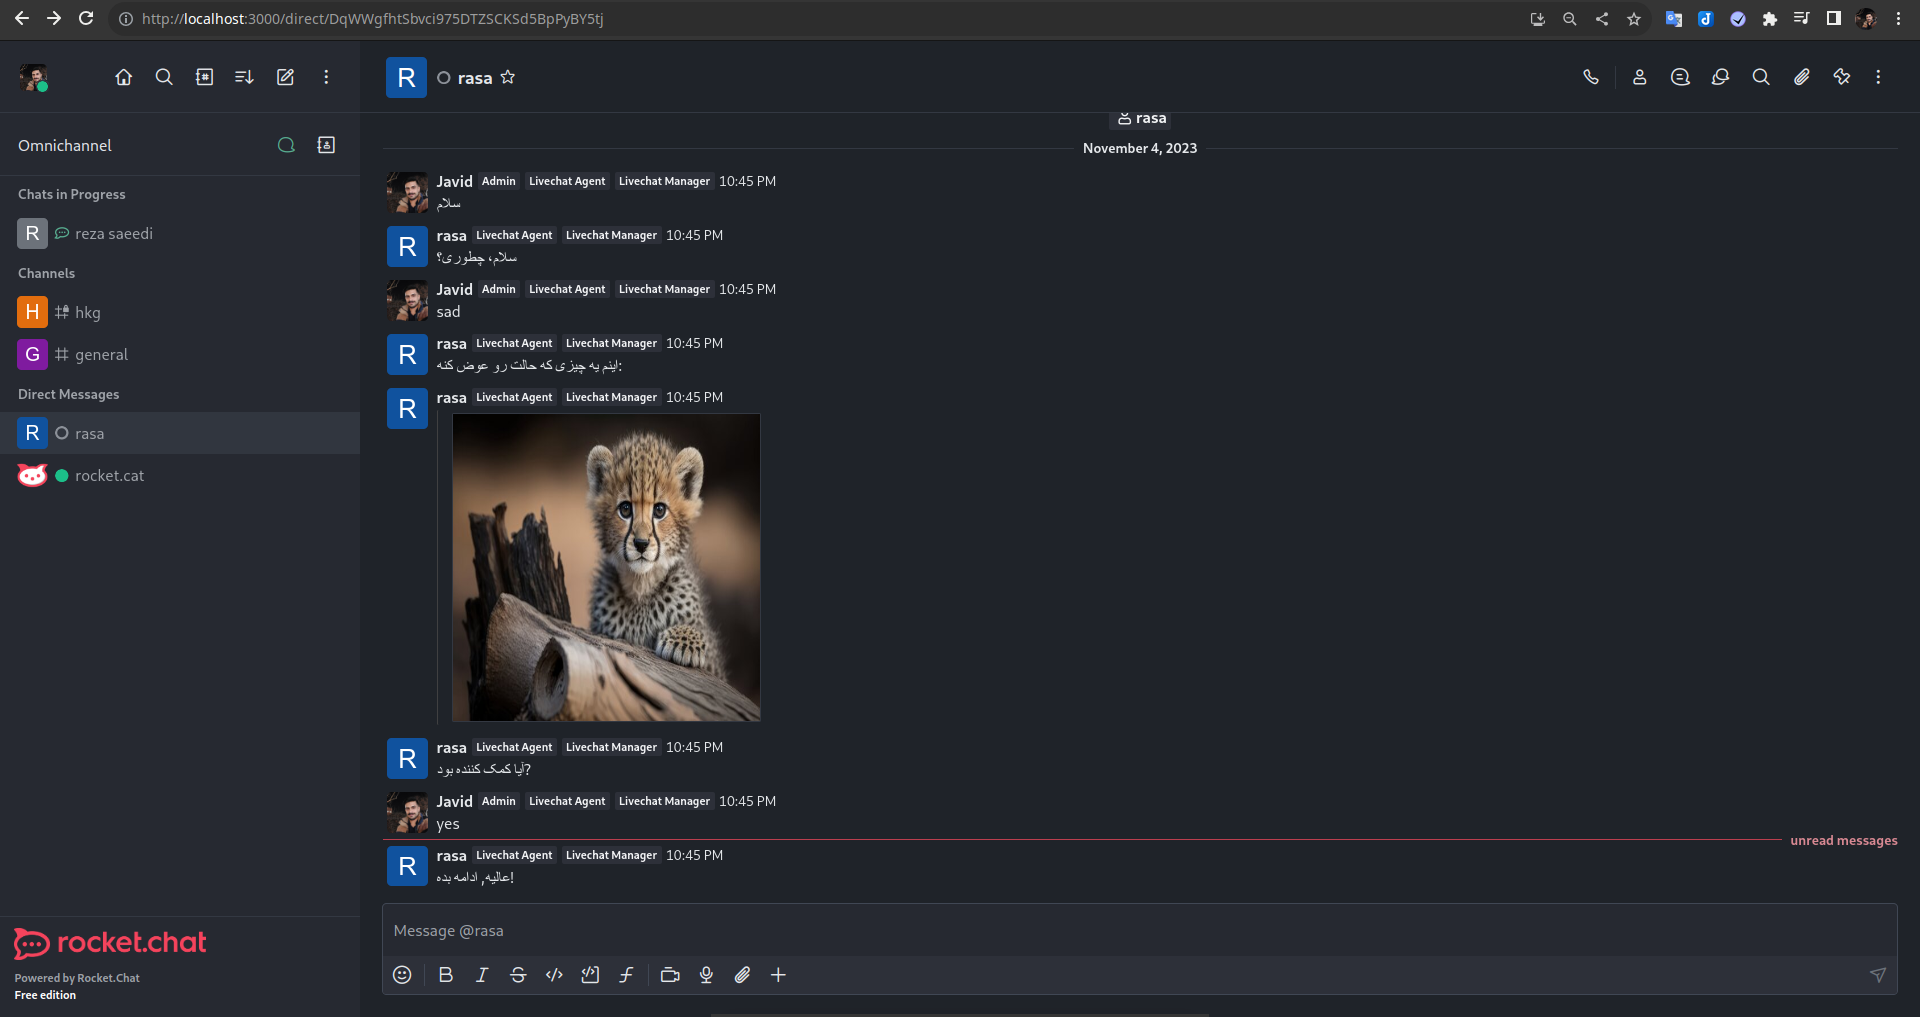
\includegraphics[width=\linewidth]{Images/Working_Connected_Rocket.Chat_Rasa_Example.png}
    \caption{نمونه متصل شده Rasa و Rocket.Chat در حال گفتوگو در محیط Rocket.Chat}
\end{figure}

\subsubsection{اطلاعات تکمیلی}

اگر می‌خواستید که \lr{Rasa bot} بتواند به پیام هایی که به صورت خصوصی به آن ارسال می‌شود نیز پاسخ دهد می‌توانید از تنظیمات زیر استفاده کنید.

\begin{latin}
    \begin{minted}[
    framesep=2mm,
    baselinestretch=1.2,
    bgcolor=LightGray,
    fontsize=\footnotesize,
    linenos,
    breaklines
    ]{bash}
    Event Trigger: Message Sent
    Enabled: True
    Channel: all_direct_messages
    URLs: http://bot_rasa:5005/webhooks/rocketchat/webhook
    Post as: bot_rasa
    \end{minted}
\end{latin}


\newpage